\chapter{Anforderungen an den Sequencer}
%TODO wie wurden ziele ausgearbeitet
\section{Formulierung der Anforderungen}
Im folgenden Kapitel werden die Anforderungen an den \textit{Sequencer} beschrieben.
Die Kapitel \textit{Ziele}, \textit{Nicht Ziele} und \textit{Test Cases} beschreiben die Anforderungen auf verschiedene Arten.
In \textit{Ziele} und \textit{Nicht Ziele} wird abstrakt beschrieben, welche Funktionen der neue \textit{Sequencer} beinhalten, beziehungsweise nicht beinhalten muss.
Im Kapitel \textit{Test Cases} werden verschiedene Fälle beschrieben die mit dem neuen \textit{Sequencer} möglichst elegant gelöst werden sollen.



\section{Ziele}
\subsection{Einfaches Interface für den Applikationsentwickler}
Mit dem bestehenden Sequencer sind vertiefte Programmierkenntnisse notwendig, um eine Sequenz zu erstellen, oder abzuändern.
Sequenzen sind nicht intuitiv verständlich.
Es werden Kenntnisse vom \textit{Control System} und dem \textit{Safety System} benötigt, um einen neuen Ablauf für den Roboter schreiben zu können. %TODO Satz
Zur Zeit werden Sequenzen von den Steuerungsentwickler geschrieben.
Wenn der Roboter fertig entwickelt worden ist, soll er an einen Kunden übergeben werden können.
Der Kunde, oder der Betreiber des Roboters, soll dann Änderungen im Ablauf des \textit{Sequencers} vornehmen können, ohne dass er vertiefte Kenntnisse von der Programmiersprache C++ oder von der inneren Funktionsweise des Roboters haben muss.
Dafür ist es notwendig, dass der Steuerungsentwickler den Roboter so abstrahiert, dass die Sequenzen aus logischen und verständlichen Schritten bestehen.


\subsection{Flexibel einsetzbar für verschiedenste Arten von Roboter}
Auch wenn die Sequenzen möglichst einfach aufgebaut werden sollen, muss der \textit{Steuerungsentwickler} für alle möglichen arten von Robotern Sequenzen bauen können.
Alle möglichen Arten von Roboter haben verschiedene Anforderungen.
Das \textit{Control System} von einem Roboterarm mit sechs Freiheitsgraden unterscheidet sich stark von einer Fertigungsstrassen mit mehreren Förderbändern.
Trotz diesen Unterschieden soll es möglich sein, für beide Arten von Robotern sinnvolle Sequenzen zu erstellen.
Das bedeutet, dass der \textit{Steuerungsentwickler} möglichst viele Freiheiten behält, ohne dass er durch das \textit{Framework} unnötig begrenzt wird.
%TODO ss missbraucht


\subsection{Parallele und blockierende Sequenzen}
Wie bereits im bestehenden Sequenzer verwirklicht wurde, sollen Sequenzen blockierend und nicht-blockierend aufgerufen werden können.
Diese Funktion von blockierenden und parallel ausgeführten Sequenzen soll auch im neuen \textit{Sequencer} beibehalten werden.
 

\subsection{Exception Handling}
Eine \textit{Exception} ist ein Ereigniss, dass nicht immer auftritt, aber auftreten kann.
Zu solchen \textit{Exception}, oder Ausnahmen, gehören zum Beispiel:
\begin{enumerate}
\item Ein blockiertes Förderband
\item Ein Timeout
\item Der Roboter soll ein Paket abholen, dass nicht vorhanden ist
\end{enumerate}
Solche Ausnahmen sollen im \textit{Sequencer} erkennt werden können und flexibel darauf reagiert werden können.
Eine solche Reaktion könnte eine spezielle Sequenz sein, die versucht, eine solche Ausnahme zu behandeln.
Alternativ soll aber auch die aktuelle Sequenz abgebrochen, oder neu gestartet werden können.


\subsection{Zugriff auf Control System}
Der aktuelle \textit{Sequencer} nutzt ein Pointer auf das \textit{Control System} um Blöcke direkt auslesen und schreiben zu können.
Wenn das \textit{Control System} betrachtet wird, kann nicht festgestellt werden, welche Blöcke vom \textit{Sequencer} ausgelesen oder geschrieben werden.
Ein klares Interface zum \textit{Sequencer} wäre wünschenswert, um das \textit{Control System} übersichtlicher zu machen.


\subsection{Safety System entlasten}
Eine Analyse von bestehenden Implementationen des alten \textit{Sequencers} hat gezeigt, dass das \textit{Safety System} viele Aufgaben übernimmt, welche besser vom \textit{Sequencer} übernommen werden sollten.
Das \textit{Safety System} sollte möglichst nur eingesetzt werden, um das System zu überwachen.
Alle anderen Aufgaben sollen vom \textit{Sequencer} oder vom \textit{Control System} übernommen werden.



\section{Nicht Ziele}
\subsection{Echtzeit}
Das \textit{Control System} und das \textit{Safety System} laufen beide in einem Echtzeit-Task.
Der \textit{Sequencer} soll aber bewusst nur mit normaler Priorität laufen und besitzt keine Echtzeit Fähigkeit.
Da der \textit{Sequencer} keine Regelung berechnet, benötigt er keine Echtzeit Fähigkeit.
Eine niedrigere Priorität als das \textit{Control System} und das \textit{Safety System} ist notwendig, dass die beiden Systeme nicht vom \textit{Sequencer} beeinträchtigt werden.


\subsection{Pfadplanung}
Die Pfadplanung ist nicht Teil des \textit{Sequencers}, da sie den Rahmen dieser Arbeit sprengen würde.



\section{Test Cases}
\subsection{Einleitung}
Die Testfälle sind so aufgebaut, dass sie möglichst einfach  und elementar sind.
Jeder \textit{Test Case} beschreibt eine andere Anforderung oder Spezialfall an den \textit{Sequencer}.
Alle in der Realität vorkommenden Situation sollte durch einen, oder einer Kombination von mehreren, \textit{Test Cases} beschrieben werden können.

Eine Ausnahme dazu bildet \textit{Test Case 8}.
In diesem Testfall wurden möglichst viele verschiedene Situationen vereint.

Mit dem \textit{Sequencer} sollen alle Testfälle sauber und verwirklicht werden werden können.


\subsection{Test Case 1: Achse einfach}
\textbf{System}
\begin{itemize}
\item Eine Achse die sich nach links und rechts bewegen kann
\item An beiden Enden befindet sich ein Endschalter
\item Ein Taster \textit{Taster links}, der die Achse nach links laufen lässt
\item Ein Taster \textit{Taster rechts}, der die Achse nach rechts laufen lässt
\end{itemize}

\textbf{Aufgabe}
\begin{itemize}
\item Solange \textit{Taster links} gedrückt bleibt, fährt die Achse nach links
\item Solange \textit{Taster rechts} gedrückt bleibt, fährt die Achse nach rechts
\item Die Achse hält an, wenn einer der beiden Endschalter erreicht wird
\end{itemize}

\textbf{Herausforderungen}
\begin{itemize}
\item Der \textit{Sequencer} muss die Eingänge \textit{Taster links}, \textit{Taster rechts} und die beiden Enschalter permanent überwachen und auf eine Änderung reagieren.
\end{itemize}


\subsection{Test Case 2: EEDURO Delta Roboter Maus}
\textbf{System}
\begin{itemize}
\item EEDURO Delta Roboter mit Maus
\end{itemize}

\textbf{Aufgabe}
\begin{itemize}
\item Während dem Idle Zustand wird auf einen Input von der Maus gewartet
\item Wenn sich die Maus für fünf Sekunden nicht bewegt, wird eine blockierende \textit{Autor-Sort Sequenz} gestartet
\item Bewegt sich die Maus innerhalb von fünf Sekunden, dann bewegen sich die Achsen entsprechend der Mausbewegung und der 5-Sekunden-Timer wird neu gestartet
\end{itemize}

\textbf{Herausforderungen}
\begin{itemize}
\item Timeout
\item Blockierende Sequenz
\end{itemize}


\subsection{Test Case 3: Rendezvous}
\textbf{System}
\begin{itemize}
\item Greifer Zubringer
\item Greifer Abholer
\item Paket: Gegenstand, der übergeben wird
\item Förderband Zubringer: Hält ständig ein neues Paket bereit für \textit{Greifer Zubringer}
\item Förderband Abholer: Transportiert ständig alle Pakete weg, welche vom \textit{Greifer Abholer} abgelegt werden
\end{itemize}

\textbf{Ablauf}
\begin{enumerate}
\item Der \textit{Greifer Zubringer} holt ein neues Paket vom \textit{Förderband Zubringer}
\item Der \textit{Greifer Zubringer} bringt das Paket in Rendezvous-Position
\item Der \textit{Greifer Abholer} übernimmt das Paket vom \textit{Greifer Zubringer} 
\item Der \textit{Greifer Abholer} legt das Paket auf das \textit{Förderband Abholer}
\end{enumerate}

%\begin{figure}[!ht]
\begin{figure}[]
\centering
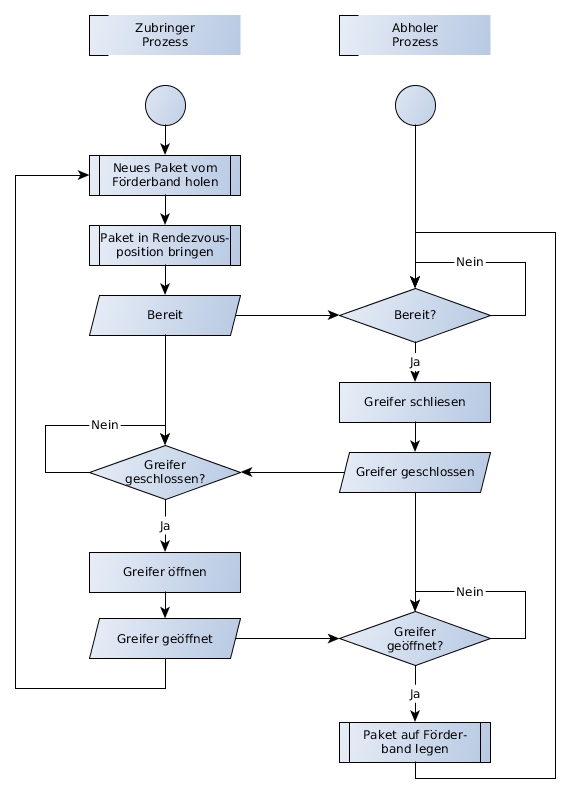
\includegraphics[angle=0,height=10cm]{images/Testcase03.png}
\caption{Ablaufdiagramm vom \textit{Test Case 3}}
\label{Testcase03Picture}
\end{figure}

\textbf{Herausforderungen}
\begin{itemize}
\item Synchronisation von zwei parallel laufenden Sequenzen
\item Kommunikation zwischen zwei Sequenzen
\end{itemize}


\subsection{Test Case 4: Sequenz pausieren}
\textbf{System}
\begin{itemize}
\item Roboterarm
\item Ein Taster \textit{Taster Pause}, der die Sequenz pausiert
\end{itemize}

\textbf{Ablauf}
\begin{itemize}
\item Der Roboterarm führt eine sich wiederholende Sequenz endlos aus
\item Wird \textit{Taster Pause} gedrückt, pausiert die Sequenz
\item Wird \textit{Taster Pause} erneut gedrückt, wird die Sequenz fortgeführt
\end{itemize}

\textbf{Herausforderungen}
\begin{itemize}
\item Jede Sequenz muss jederzeit pausiert werden können
\item Der Taster gibt nur einen Impuls, nicht eine bleibende Pegeländerung an einem Eingang
\item Timeouts müssen pausiert werden
\end{itemize}


\subsection{Test Case 5: Zwei Roboterarme}
\textbf{System}
\begin{itemize}
\item Roboterarm A
\item Roboterarm B
\item Ein Taster \textit{Taster Pause}, der beide Sequenzen pausiert
\end{itemize}

\textbf{Ablauf}
\begin{itemize}
\item Beide Roboterarme führen sich wiederholende Sequenz endlos aus
\item Wird \textit{Taster Pause} gedrückt, pausieren beide Sequenzen
\end{itemize}

\textbf{Herausforderungen}
\begin{itemize}
\item Zwei parallel laufende Sequenzen müssen mit einem Taster pausiert werden können
\end{itemize}


\subsection{Test Case 6: Prellender Taster}
\textbf{System}
\begin{itemize}
\item Ein prellender Taster \textit{Taster A}
\end{itemize}

\textbf{Aufgabe}
\begin{itemize}
\item Ein prellender Taster soll sauber eingelesen werden
\end{itemize}

\textbf{Herausforderungen}
\begin{itemize}
\item Der Taster muss entprellt werden
\item Mehrmaliges drücken soll sauber registriert werden, auch wenn der Taster in schneller Abfolge gedrückt wird
\end{itemize}

\begin{figure}[]
\centering
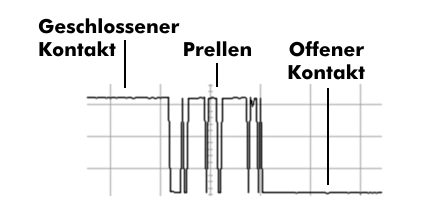
\includegraphics[angle=0]{images/Testcase06.png}
\caption{Signalverlauf bei einem prellenden Schalter}
\label{Testcase06Picture}
\end{figure}


\subsection{Test Case 7: Menü}
\textbf{System}
\begin{itemize}
\item Ein beliebige Anzahl Taster \textit{Taster A}, \textit{Taster B}, \textit{Taster C}, ....
\end{itemize}

\textbf{Aufgabe}
\begin{itemize}
\item Wenn sich das System in einem \textit{Idle} Zustand befindet, soll jeder Taster eine andere Sequenz starten
\end{itemize}

\textbf{Herausforderungen}
\begin{itemize}
\item Dieses \textit{Menü} lässt sich nicht im klassischen Sinne als eine Sequenz, also eine Abfolge von Schritten, beschrieben werden. Trotzdem soll eine einfache Implementierung im \textit{Sequencer} möglich sein
\end{itemize}


\subsection{Test Case 8: Detailliertes Rendezvous}
Dieser \textit{Test Case} basiert auf auf dem \textit{Test Case 3}.

asdf \ref{sec:anhang_test_case_8}

asdf \ref{TestCase8Sequence1Picture}
